% !TEX root = mythesis.tex

%==============================================================================
\chapter{Auswertung}
\label{sec:auswertung}
%==============================================================================

Nachdem die Simulationen fertiggestellt wurden, sollen hier die gewonnenen Daten
ausgewertet werden, mit der Motivation am Ende das statische Potential des
Quark-Antiquark-Paares zu extrahieren.

\section{Energie und durchschnittliche Plaquette}
Um zunächst ein Gefühl für die Thermalisierung (also das Erreichen des
Gleichgewichtszustands) des Gitters zu bekommen, wurde zwischen den Sweeps zunächst
die Gesamtenergie
\[
    E = \sum_{x \in \Lambda} \sum_{\mu < \nu} \text{Re} \; \text{tr}~U_{\mu \nu}(x)
\]
vermessen, woraus sich auch die durchschnittliche Plaquette
\[
    P = \frac{E}{6 L_t L_s^3 N_\mathrm{c}}
\]
berechnen lässt. Das Ergebnis ist in Abhängigkeit von der Sweepzahl in Abb.
\ref{fig:avgPlaquette} dargestellt. Wie man erkennen kann, wurde das System kalt, d.\,h.
mit $U_\mu(x) = \mathds{1} \forall U_\mu(x) \in \mathcal{U}$ initialisiert, daher
beginnen die Werte bei $P = 1$. In unter 20 Sweeps konvergiert das System dann zu
einem stabilen Plateau. Nun kann der Erwartungswert von $P$ approximiert werden.
Dazu wird wie beim harmonischen Oszillator das arithmetische Mittel und der
Standardfehler von vielen Messwerten von $P$ gebildet. Hier wurden insgesamt
10000 Sweeps durchgeführt. Für $\beta = 1$ erhalten wir
\[
    \overline{P} = 0.24308 \pm 0.00010.
\]
Dieser Wert allein ermöglicht zwar den Vergleich mit vorherigen Simulationen, bietet
allein aber wenig Einblicke in die Physik. Dazu bieten erst die Wilson-Loops
mehr Gelgenheit.

\begin{figure}[htbp]
    \centering
    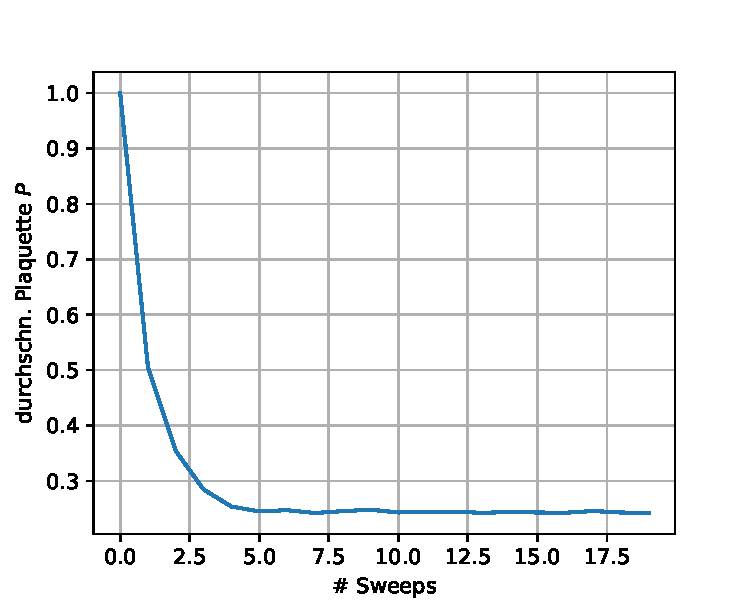
\includegraphics[width=.7\textwidth]{avgPlaquette}
    \caption{Die durchschnittliche Plaquette eines $16 \times 8^3$-Gitters bei
    $\beta = 1$ als Funktion der Iterationszahl: Nach ca. 5 Sweeps scheint das System
    bereits einen Gleichgewichtszustand zu erreichen.}
    \label{fig:avgPlaquette}
\end{figure}

\section{Vermessen von Wilson-Loops verschiedener Größe}

\begin{figure}[htbp]
    \centering
    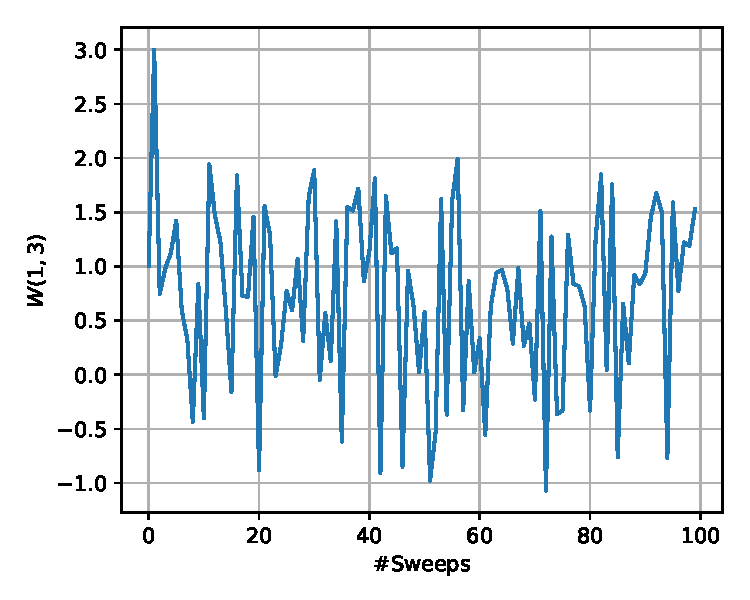
\includegraphics[width=.4\textwidth]{1x3loop}
    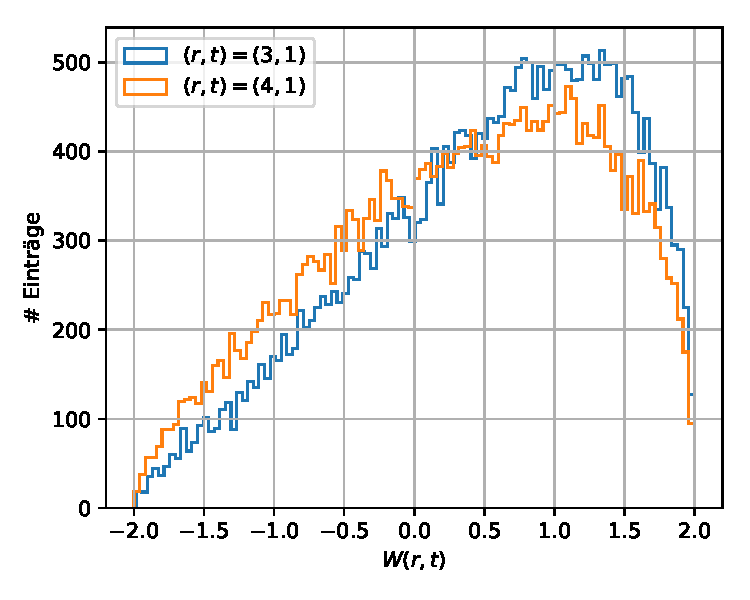
\includegraphics[width=.4\textwidth]{1x3and4histogram}
    \caption{Links: Alle Messwerte eines $1 \times 3$-Wilson-Loops. Rechts:
    Verteilung relevanter Messwerte (nach Equilibrierung alle 5 sweeps gemessen).}
    \label{fig:singleLoops}
\end{figure}

Als Nächstes wurden also planare und nicht-planare Wilson-Loops, also rechteckigen
geschlossenen Ringen von Paralleltransporten betrachtet. Zunächst
wurden Loops wie in Abschn. \ref{sec:thWilsonLoops} definiert zwischen den Sweeps
vermessen. Als Bsp. sind die Messwerte für einen $1 \times 3$-Loop als Funktion der
Sweepzahl in Abb. \ref{fig:singleLoops} dargestellt. Zuerst fällt auf, dass die
Messwerte sehr stark zwischen den Werten $\pm 2$ fluktuieren. Deswegen sind viele
Messwerte zur zuverlässigen Bestimmung des Erwartungswertes notwendig. In
\ref{fig:singleLoops} ist die Verteilung der Messwerte
für zweimal 29800 Messungen dargestellt. Wieder ist zu erkennen, dass die Verteilung
sehr \enquote{breit} ist, und das insbes. für die Unterscheidung der verschiedenen
Messungen viele Messungen notwendig sind, um den Standardfehler auf $\overline{W(r,t)}$
entsprechend zu drücken. In diesem konkreten Fall wurde
\[
    \overline{W(3,1)} = 0.4984 \pm 0.0030, \;
    \overline{W(4,1)} = 0.3270 \pm 0.0032
\]
berechnet. Bemerkenswert ist, dass der Standardfehler in diesem Bsp. und bei allen
Messungen (unabhängig von der Größe der Schätzer) ungefähr gleich groß ist. Dies
ist vermutlich auf die Ähnlichkeit der Verteilung (und somit der Standardabweichung)
und der gleichen Anzahl von Samples zurückzuführen. (Der Standardfehler skaliert mit
$\frac{\sigma}{\sqrt{N}}$.)

\section{Extrahierung der Werte für das statische Potential}

\begin{figure}[htbp]
    \centering
    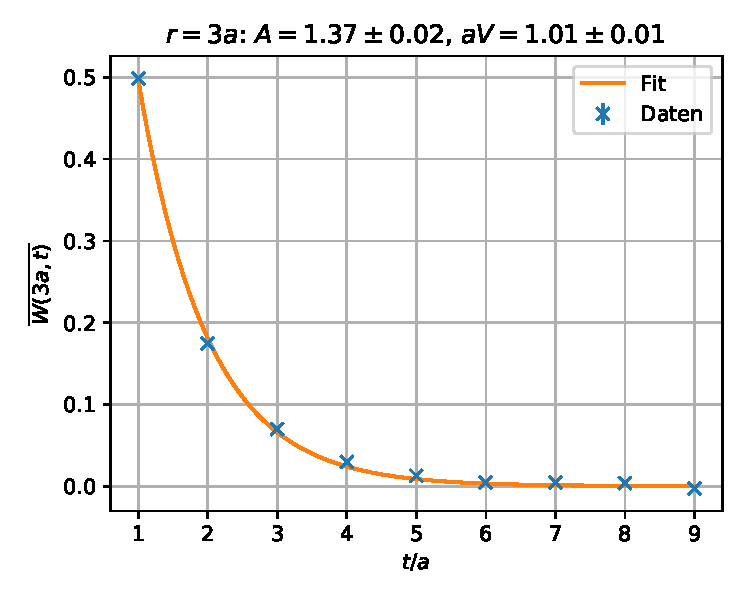
\includegraphics[width=.7\textwidth]{loopResultsBeta23r3.pdf}
    \caption{Beispiel für Wilson-Loop-Messwerte zur Bestimmung des statischen
    Potentials für $r = 3a$. Verwendetes Modell:
    $\overline{W(3a,t)} = A \cdot \exp(-aV t/a)$.}
    \label{fig:loopResultr3}
\end{figure}

Grundlage für die Berechnung des Wertes des statischen Potentials für ein festes
$r$ bietet die Relation \eqref{eq:wilsonStaticPot}. Ziel ist, aus den Daten eine
Abhängigkeit $aV(r)$ zu gewinnen. Zunächst wurde also der
Erwartungswert $\overline{W(r,t)}$ in Abhängigkeit von $t$ betrachtet
Abb. \ref{fig:loopResultr3} exemplarisch für $r = 3a$ dargestellt ist. Dies sollte
eine abklingende Exponentialkurve liefern, deren Exponentialkoeffizient dann dem
statischen Potential bei einem Abstand $r=3a$ entspricht. Der exponentielle
Zusammenhang ist klar erkennbar, ein Fit liefert den gewünschten Parameter
$a V(r)$. ($t$ ist natürlich nur bis auf die Gitterkonstante $a$ bestimmt.) Es
fällt aber auch auf, dass die Messwerte bei größeren $t$ nicht mehr allzu klar
dem exponentiellen Zusammenhang folgen. Natürlich macht sich die Tatsache, dass
der statistische Fehler immer ungefähr gleich groß ist, besonders bei kleinen
Messwerten bemerkbar.

\section{Confinement?}

\begin{figure}[htbp]
    \centering
    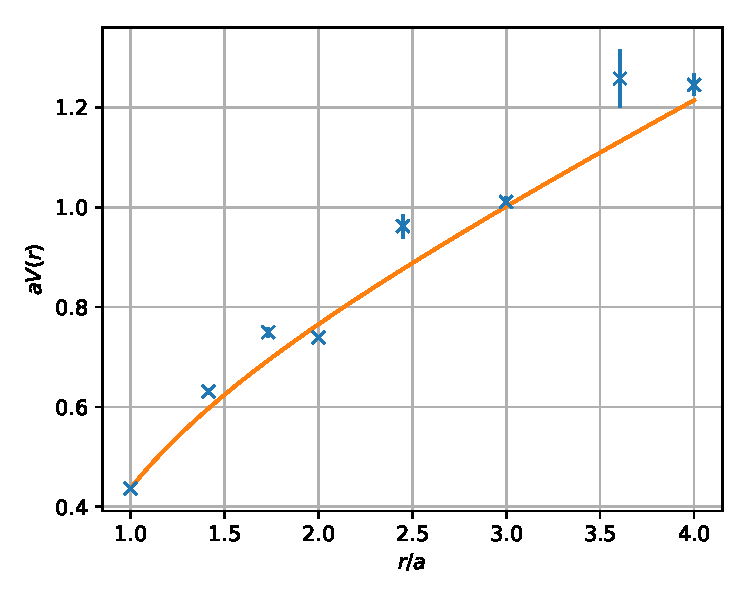
\includegraphics[width=.7\textwidth]{aVfitBeta23.pdf}
    \caption{Das statische Potential in Abhängigkeit vom Abstand von Quark und
    Antiquark: Es ist klar ein linearer Zusammenhang erkennbar.}
    \label{fig:aVfit}
\end{figure}

Die oben beschriebene Messung von $\overline{W(r,t)}$ wurde für
$(r, t) \in \{1, \sqrt{2} \approx 1.4, \sqrt{3} \approx 1.7, 2, \sqrt{6} \approx 2.4,  3, \sqrt{13} \approx 3.6, 4\} \times \{1,2,3,4,5,6,7,8,9\}$
durchgeführt. Für die verschiedenen $r$-Werte wurde nach dem beschriebenen
Verfahren $a V(r)$ bestimmt. Das Resultat ist in Abb. \ref{fig:aVfit} dargestellt.
Die Schlussfolgerung ist klar: Das Potential enthält deutlich einen linearen Term.
Passt man eine Funktion der Form
\[
    a V(r) = -\frac{A}{r} + B + \sigma \cdot r
\]
an die Daten ab, so erhält man
\[
    \sigma = (0.189\pm 0.010) \frac{1}{a}
\]
für die sog. string tension\footnote{Das Potential hat Dimension $L^{-1}$,
dementsprechend ist in der hier gewählten Form $[\sigma] = L^{-1}$.}. Es fällt auf,
dass die Fitkurve nur zwei Fehlerbalken der Datenpunkte direkt schneidet
($\chi^2 = 16.6$). Dies
könnte zweierlei Gründe haben: Auf der einen Seite könnten die Fehler unterschätzt
werden. Diese wurden über den Standardfehler auf das arithmetische Mittel abgeschätzt.
Hier böten andere Methoden (e.\,g. Bootstrap) ggf. bessere Abschätzungen des Fehlers.
Auf der anderen Seite fällt bei genauerer Betrachtung auf, dass die vier Datenpunkte
für ganzzahliges $r/a$ fast perfekt auf einer Linie liegen. Die Datenpunkte für
nichtganzzahlige $r/a$ weichen hiervon ab, da sie von der gewählten Form der
nichtplanaren Loops abhängen. Hier könnte man dadurch Abhilfe schaffen, dass man
verschiedene Formen für die nichtplanaren Wilsonloops vermisst und am Ende über 
die Ergebnisse mittelt. Insgesamt kann aber trotzdem ein linearer Zusammenhang
erkannt werden.

Nun stellt sich natürlich die Frage nach den physikalischen Implikationen dieses
Ergebnisses. Zunächst ist festzustellen, dass die SU(2)-Symmetrie keine alleinige
Wurzel der bekannten Wechselwirkungen darstellt. Insofern kann die gewonnene
Erkenntnis nur in ihrem Analogon zur SU(3)-Symmetrie und der daraus
\enquote{gewonnenen} Quantenchromodymanik verstanden werden. Klar ist: Für die
Parameter $\beta = 2.3$ und $N_\text{t} = 10$ konnte Confinement nachgewiesen
werden. Interpretiert man das untersuchte Gitter als ein tatsächliches
Kristallgitter im Rahmen der statistischen Mechanik (die durchgeführten
Simulationen sind hierzu äquivalent), so kann man das gewonnene Ergebnis als Teil
eines Phasenüberganges bei endlicher Temperatur betrachten. In diesem Fall ist die
Temperatur durch $\theta = \frac{1}{N_\text{t}}$ gegeben und die zwei Phasen
lassen sich als \enquote{Confinement} ($\theta$ klein) und \enquote{Deconfinement}
($\theta$ groß) klassifizieren.

%Nun stellt sich natürlich die Frage nach den physikalischen Implikationen dieses
%Ergebnisses. Die SU(2)-Symmetrie ist nicht alleinige Wurzel einer einzelnen
%Wechselwirkung, vielmehr wird sie im Rahmen der Vereinigung der elektromagetischen
%mit der schwachen Wechselwirkung verwendet, die von SU(2)$\times$U(1) generiert
%wird. Diese Vereinheitlichung ist jedoch erst oberhalb einer bestimmten
%Energieskale resp. unterhalb einer bestimmten Längenskale sinnvoll. Gleichzeitig
%ist zu beachten, dass Confinement aufgrund der laufenden Kopplung nur bei
%kleinen Energien, i.\,e. großen Kopplungen auftritt. (Dies gilt auch für SU(3)
%und die starke Wechselwirkung: Hier spricht man im Gegensatz zu Confinement bei
%kleinen Energien von \emph{asymptotischer Freiheit} bei großen Energien, wo die
%Kopplung schwächer wird und Quarks nur noch leichtinteragierend sind.) Diese beiden
%Erkenntnisse zusammengenommen, ist zu schlussfolgern, dass bei den für die Realität
%relevanten Energieskalen Confinement nicht auftritt.
